\documentclass[tikz]{standalone}
\begin{document}
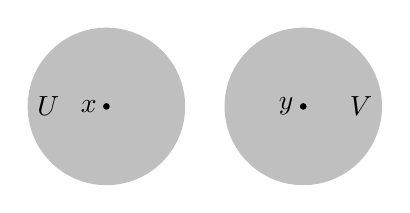
\begin{tikzpicture}
\fill[gray!50] (0,0) circle (1cm);
\node[right] at (-1,0) {\(U\)};
\fill (0,0) circle(1.2pt) node[left] {\(x\)};
\fill[gray!50] (2.5,0) circle (1cm);
\node[left] at (3.5,0) {\(V\)};
\fill (2.5,0) circle(1.2pt) node[left] {\(y\)};
\end{tikzpicture}
\end{document}
